\subsection{Sikker kommunikation}
Der vil i dette afsnit blive kigget på hvad det vil sige at kommunikere sikkert, både i levering, men også i håndteringen af kommunikationen. Tilsidst vil der blive konkluderet et grundlag for foretagelse af sikker kommunikation.

\subsubsection{Kryptologi}
De fleste forbinder moderne IT-sikkerhed med avanceret krypteringsalgoritmer. Selvom dette er en vigtig del af IT-sikkerhed, er det dog ikke den eneste måde at sikre kommunikation på. Under emnet kryptologi, som omhandler alle former for hemmelig kommunikation, er kryptografi kun en del af emnet. Et andet vigtigt koncept som også dækker er steganografi, der videre vil blive diskuteret i næste afsnit. Den førnævnte algoritmebaseret sikring af data falder ind under kryptografi. Eksempler på disse spænder fra den simpleste alfabet skiftende algoritme, f.eks. ét bogstav skift til højre, og videre til moderne hashing algoritmer. Fælles for anvendelsen af alle disse er dog, at det tydeligt viser en intention om at hemmeligholde indholdet. Hermed kan selve krypteringen gøre beskeden mistænkelig, da information af lav værdi ikke ville være besværet værd.

\subsubsection{Steganografi}
Som nævnt i indledningen, består emnet kryptologi af flere underkategorier. Den kategori der vil blive fokuseret på her, er steganografi. Steganografi omhandler metoder til at skjule selve eksistensen af en given besked, i stedet for at gøre indeholdet ulæseligt, som er hvad kryptografi gør.\cite{MeningOfSteganografi} Et eksempel på beskeder der er sikret med steganografi, kunne være de hemmelige tegn og signaler, også ofte brugt af spioner i film. Et tilsyneladende tilfældigt symbol på et umiddelbart ligegyldigt sted, men blot en af de mange forskellige ting som kunne sende en besked sikkert frem. Alt dette vil foregå imens ingen andre vil opdage, at der overhovedet var en form for kommunikation. Udenfor fiktionens verden findes der dog også nogle eksempler på grupper, som har udviklet systemer baseret på steganografi til at kommunikere internt.
\begin{figure}[H]
    \begin{subfigure}{0.5\textwidth}
    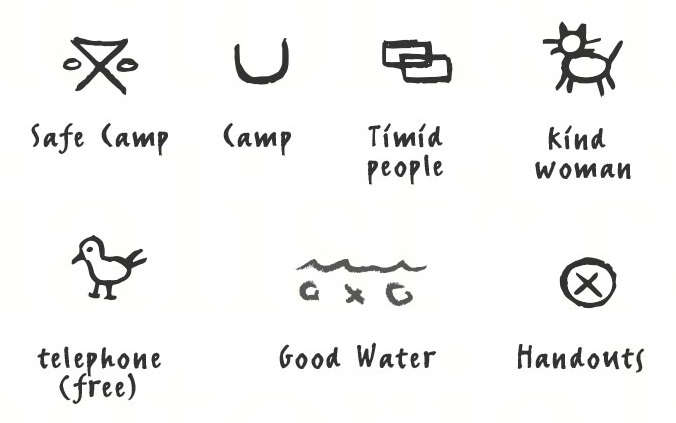
\includegraphics[width=0.9\linewidth, height=5cm]{Projectdoc/Problemanalyse/Illustrationer/hobo.jpg} 
    \caption{The Hobo Code}
    \label{fig:hobocode}
    \end{subfigure}
    \begin{subfigure}{0.5\textwidth}
    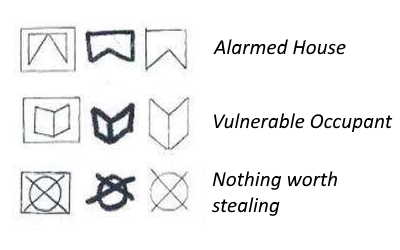
\includegraphics[width=0.9\linewidth, height=5cm]{Projectdoc/Problemanalyse/Illustrationer/da-code.png}
    \caption{Da Pinchi Code / The Burglars Code}
    \label{fig:burglarscode}
    \end{subfigure}
    \caption{To af de legendariske steganografi metoder}
    \label{fig:legendscode}
\end{figure}
Et kendt eksempel på sådan et steganografisk system kunne være "The Hobo Code [Se figur: \ref{fig:hobocode}]", et system kendt, og anvendt, af hjemløse til at hjælpe hinanden med deres overlevelse\cite{TheHoboCode}. Disse beskeder er aldrig rigtigt blevet dateret, og ingen i dag kender derfor deres præcise oprindelse, men det vides dog stadig at dette steganografiske system har været anvendt i flere århundrede.\\ 
Foruden videnen om metodens eksistens gennem årene, vides også at der findes flere andre ligende afarter af denne kendte kode, såsom den nytidiske "Da Pinchi Code [Se figur: \ref{fig:burglarscode}]". Denne kode bliver alment anvendt af konstruktions arbejdere, men siges også, efter historier, at have været anvendt af indbrudstyve eller andre kriminelle.\cite{DaPinchiCode} At lave sikre systemer handler dog ikke kun om den underlæggende teori. Brugerne af systemet kan også lave fejl, eller bruge systemet på ikke tiltænkte måder, som potentielt kunne skade systemet, eller brugerne, som en helhed. Derfor vil der i det næste afsnit diskuteres en sådan brugerbaseret problematik. 

\subsubsection{Brugeren som sikkerhedsbrist}
\label{Brugeren_som_sikkerhedsbrist}
I dag forsøger mange at bibeholde, hvad der for dem synes at være, sikker eller hemmelig kommunikation via diverse tjenester. For nogle er disse tjenester dog mere sikre end hos andre. Som et eksempel vil de fleste private computerbrugere, nok mene at deres generelle email er forholdsvis sikker, men deres arbejdsplads deler muligvis ikke samme overbevisning. Dette var f.eks. tilfældet hos Hillary Clintons email-skandale tilbage i 2015-2016.\cite{Hillary_Email_History} Hillary Clinton havde oprettet sin egen mailserver til håndtering af alle hendes mails, dog mener flere, blandet andet FBI, at denne handling har været en "ekstremt uforsigtigt" håndtering af hendes fortrolighed. Trods Hillarys skandale menes dog ikke at et større sikkerhedsbrud har fundet sted, men Hillary har stadig som bruger mindsket den tilgængelige sikkerhed, i følge FBI, da de mener at hun fejlagtigt har misbrugt det vante system.\cite{Hillary_Email_skandale} Det efterfølgende afsnit vil danne overblik over de vigtigste elementer af sikker kommunikation.

\subsubsection{Grundlaget for sikker kommunikation}
I dag forsøger folk ved alle tænkelige metoder at kryptere forbindelser på nettet, men da kryptering er kendt og synligt, vil det derfor på et eller andet tidspunkt blive, eller være forsøgt, brudt. Steganografiske metoder har til gengæld alle den vigtige egenskab, at ikke alle vil ligge mærke til dem, selvom de befinder sig lige foran dem. Steganografiens egenskaber kan sammen med de sociale mediers endeløse strøm af indhold, fungere som et ekstra lag af sikkerhed. Udover kommunikationens skjulte eksistens, vil den kommunikation være at finde blandt milliarder af uskyldige indlæg.\\
En effektiv implementation af dette, kunne endda sikre kommunikation imellem stridende lande, hvor sikker og åben kommunikation ikke er en selvfølge.
Dog skal man også, for en endelig metode, have i tanke, at jo mere frihed man giver en bruger, jo større er risikoen for, at brugeren anvender systemet på en ikke tiltænkt, eller ligefrem uforsvarlig måde.
\\\\
I det næste afsnit vil nogle udvalgte kommunikationsplatforme blive analyseret baseret på netop disse kriterier.